\section{Some Statistics}

Once compiled in JavaScript it is possible to run with \textit{NodeJs} in the terminal. I have therefore exploited this possibility to launch the algorithms over some chosen \textit{Regular Expression} to test the Learners' performances. Some statistics between the two algorithms are proposed in paper \cite{NLPaper}: Bollig \textit{et al.} counts the number of states of the final automata given by the Learners and accepted by the Teacher along with the number of membership and equivalence queries. I added some personal criteria of comparison in order to also see how many time the \textit{Observation Table} is found not close or not consistent (I will call them closedness and consistence problems) and the number of transition of the automata.

All of these statistics can be obtained by executing the files into the \textit{test\_nodejs} folder. The script creates a CSV file in which all the comparison values are stored and then a \textit{Python} file can parse the CSV to finally transform the resulting CSV into plots\footnotetext{To display plots I used the \textit{matplotlib} library}.

The statistics aim to see the strength and the weaknesses of the to Learners, therefore I have tested them over specific \textit{Regular Expressions (RegEx)}. These \textit{RegEx} take into account the size of the \textit{cRFSA}: since it \textit{can} be exponentially smaller than the size of the \textit{mDFA}.

\subsection{The cRFSA is exponentially smaller then the mDFA}
Languages recognizing by the \textit{RegEx} $\U = (a+b)^*a(a+b)^n$ for a chosen $n$ are known to build \textit{mDFA} whose number of states increase exponentially every time we increase the value of $n$. It is also known that these same \textit{RegEx} can be represented by \textit{non-deterministic} automata (\textit{NFA}) whose number of state grows linearly with $n$. Moreover if we analyze the language recognized by every state of these automata represent exactly all of the \textit{prime} residuals of $\U$. So we can intuitively understand that $U$ can be also represented by a \textit{cRFSA} which has the same number of state as the \textit{NFA}.

\begin{figure}[!htb]
  \centering
  \begin{subfigure}[b]{0.3\textwidth}
    \includegraphics[width=\textwidth]{../statistics/plots/wrostDFA/State nb in A.png}
    \caption{Comparing State Number}
    \label{fig:StateWrostDFACompare}
  \end{subfigure}
  \begin{subfigure}[b]{0.3\textwidth}
    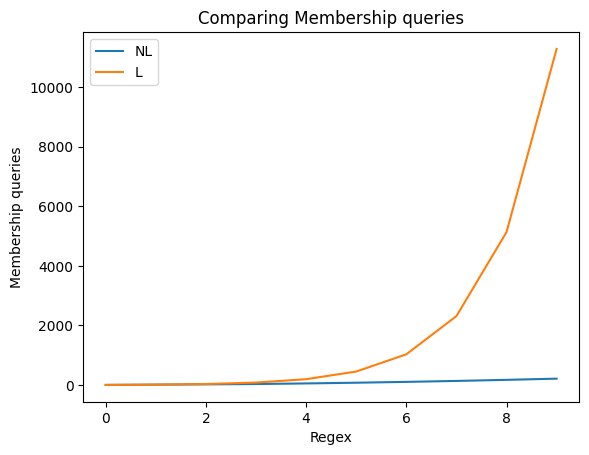
\includegraphics[width=\textwidth]{../statistics/plots/wrostDFA/Membership queries.png}
    \caption{Membership queries Number}
    \label{fig:MemberWrostDFACompare}
  \end{subfigure}
  \begin{subfigure}[b]{0.3\textwidth}
    \includegraphics[width=\textwidth]{../statistics/plots/wrostDFA/Equivalence queries.png}
    \caption{Equivalence queries Number}
    \label{fig:EquivWrostDFACompare}
  \end{subfigure}
  \begin{subfigure}[b]{0.3\textwidth}
    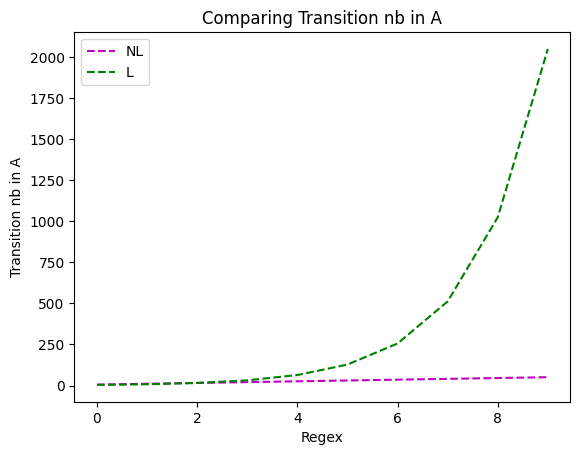
\includegraphics[width=\textwidth]{../statistics/plots/wrostDFA/Transition nb in A.png}
    \caption{Transition Number}
    \label{fig:TransitionWrostDFACompare}
  \end{subfigure}
  \begin{subfigure}[b]{0.3\textwidth}
    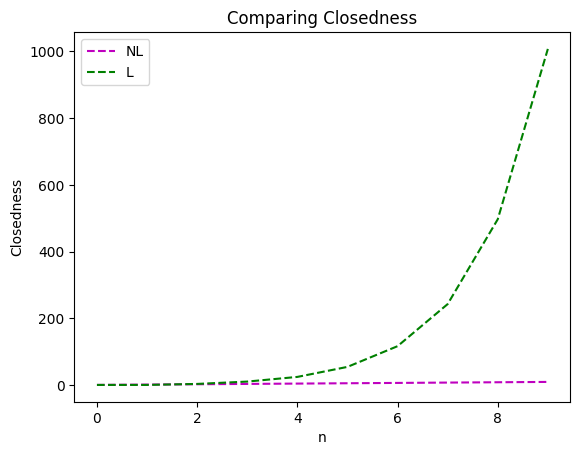
\includegraphics[width=\textwidth]{../statistics/plots/wrostDFA/Closedness.png}
    \caption{Closedness Problem Number}
    \label{fig:ClosednessWrostDFACompare}
  \end{subfigure}
  \begin{subfigure}[b]{0.3\textwidth}
    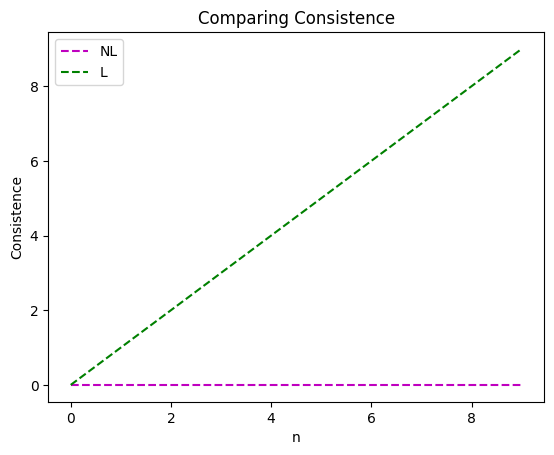
\includegraphics[width=\textwidth]{../statistics/plots/wrostDFA/Consistence.png}
    \caption{Consistence Problem Number}
    \label{fig:ConsistenceWrostDFACompare}
  \end{subfigure}
  \caption{mDFA vs cRFSA on $U = (a+b)^*a(a+b)^n)$}
  \label{fig:wrostDFA}
\end{figure}

From \cref{fig:wrostDFA}, we can see that the \textit{L*} is much more expensive than \textit{NL*}. As announced the number of states of the \textit{mDFA}'s curve is exponential compared to $n$ and that this also impact the number of transitions, membership queries and closedness problems.

An other particular plot is \cref{fig:ConsistenceWrostDFACompare} where the number of Consistence Problems grows linearly for \textit{L*} and equals zero for NL*.

Let's analyze at first L*.

Starting from $\U = (a+b)^*a(a+b)^n$. L* sends a first conjecture thinking that $\U = \varnothing$ since $\E, a$ and $b$ are not in $\U$. However the Teacher give back a counter-example of the shortest word $\omega$ belonging to $S$\footnote{The Teacher is supposed to be the \textit{Minimal Adequate Teacher}}. We have that $\omega = a^{n+1}$ and that all prefix of $\omega$ are not in $\U$. We will have that the table will not be consistent: $row(\E) = row(a^n)$ but $row(\E \cdot a) \neq row(a^n \cdot a)$. So we add the new column $a$. This new column will make $row(\E) = row(a^{n-1})$ but $row(\E \cdot a) \neq row(a^{n-1} \cdot a)$. We continue in this way $n$ times and at that moment we will have $E = \{\E, a, \dots, a^n\}$. This will stop the table to be not consistent since there will be no more similar row in $S$. Since the automaton associated to $\U$ has precisely $2^{n+1}$ states then to have $2^{n+1}$ different rows in $S$ (one for each state of the \textit{mDFA}), and knowing that after the first $n$ consistence problems, L* will have to find $2^{n+1}-n$ closedness problem to promote rows from $SA$ to $S$.

Let's now analyze the NL* behavior.

This algorithm as said in \cref{section:NL}, tries to find all prime residuals of $\U$. After the first conjecture, that, as for the L* is supposed to accept the language $\U = \varepsilon$, the Learner receives the counter-example $c = a^n$. Since \textit{NL} adds the counter-example to $E$ and so it will directly make $E = \{\E, a, \dots, a^n\}$. This coincides with the number of residuals of $\U$. In this case the  algorithms only has to promote $n$ rows, one for each residual and this is possible since the promotion of a rows will create new rows in $SA$ to respect make the \OT complete.

We can finally note that the number of equivalence queries is the same for the two algorithms since:
\begin{itemize}
  \item if $n = 0$, $U = (a+b)^*a$. In this case, the algorithms understand the language after only one equivalence query. The first five membership queries are enough to understand the language.

  \item else: the two Learners only need two equivalence queries to understand $\U$\footnote{Note that in \cref{fig:EquivWrostDFACompare} the curve of NL* and L* are superposed}. After the first equivalence query, L* and NL* receive the first counter-example and thanks to the consistence and closedness check, both algorithms will be able to send a second conjecture $\A$ where $\LA = \U$.
\end{itemize}

\subsection{The cRFSA has the same size as the mDFA}
\label{sec:worstRFSA}

In this section we are going to show the behavior of the two algorithms on a particular class of regular expressions depending on a fixed parameter $n$ where the \textit{cRFSA} has exactly the same size of the \textit{mDFA} but where the corresponding minimum \textit{NFA} is exponentially smaller.
This automaton is proposed in Section 6 of \cite{RFSA}. The construction is done for an automaton $A_n = \langle \Sigma, Q, Q_I, F, \delta \rangle $ where:
\begin{itemize}
  \item $\Sigma = {a, b}$,
  \item $Q = \{q_i \mid 0 \leq i < n-1 \}$,
  \item $Q_I = \{q_i \mid 0 \leq i < n/2\}$,
  \item $F = q_0$
  \item $\delta(q_i,a) = q_i+1$for $0 \leq i< n - 1$, $\delta(q_{n-1},a) = q_0$, $\delta(q_0,b)=q_0$, $\delta(q_i,b) = q_{i-1}$ for $1<i<n$ and $\delta(q_1,b)=q_{n-1}$.
\end{itemize}

As proved in that paper, the number of state a minimal \textit{NFA} equals $n$, but the number of states of the \textit{cRFSA} is exponential with reference to $n$.
The statistics of the execution of the two algorithms are shown in \cref{fig:wrostRFSA}.

\begin{figure}[!htb]
  \centering
  \begin{subfigure}[b]{0.3\textwidth}
    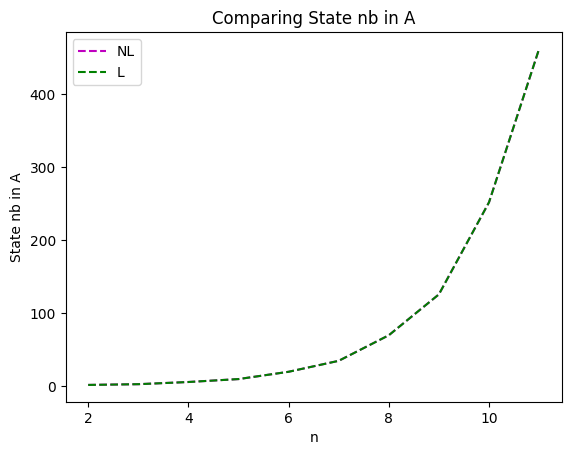
\includegraphics[width=\textwidth]{../statistics/plots/wrostRFSA/State nb in A.png}
    \caption{Comparing State Number}
    \label{fig:StateWrostRFSACompare}
  \end{subfigure}
  \begin{subfigure}[b]{0.3\textwidth}
    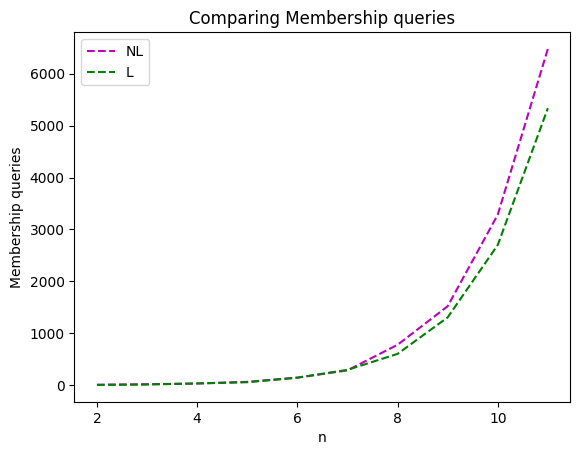
\includegraphics[width=\textwidth]{../statistics/plots/wrostRFSA/Membership queries.png}
    \caption{Membership queries Number}
    \label{fig:MemberWrostRFSACompare}
  \end{subfigure}
  \begin{subfigure}[b]{0.3\textwidth}
    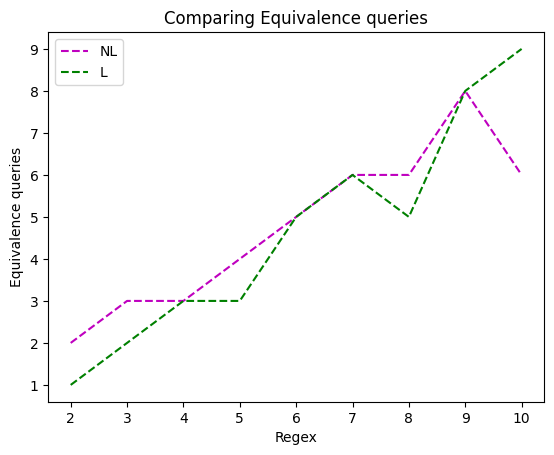
\includegraphics[width=\textwidth]{../statistics/plots/wrostRFSA/Equivalence queries.png}
    \caption{Equivalence queries Number}
    \label{fig:EquivWrostRFSACompare}
  \end{subfigure}
  \begin{subfigure}[b]{0.3\textwidth}
    \includegraphics[width=\textwidth]{../statistics/plots/wrostRFSA/Transition nb in A.png}
    \caption{Transition Number}
    \label{fig:TransitionWrostRFSACompare}
  \end{subfigure}
  \begin{subfigure}[b]{0.3\textwidth}
    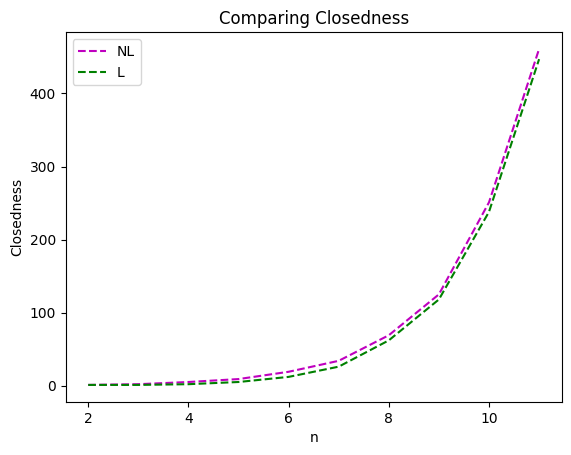
\includegraphics[width=\textwidth]{../statistics/plots/wrostRFSA/Closedness.png}
    \caption{Closedness Problem Number}
    \label{fig:ClosednessWrostRFSACompare}
  \end{subfigure}
  \begin{subfigure}[b]{0.3\textwidth}
    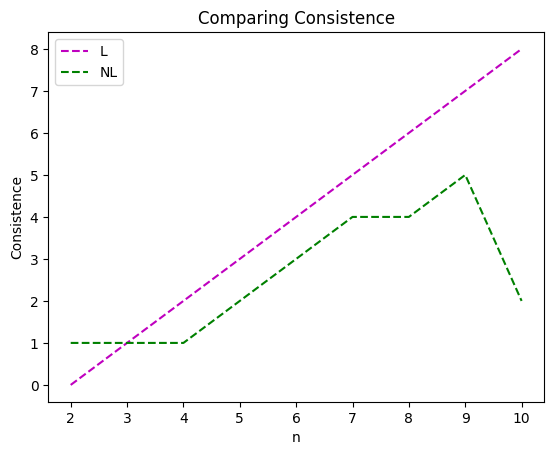
\includegraphics[width=\textwidth]{../statistics/plots/wrostRFSA/Consistence.png}
    \caption{Consistence Problem Number}
    \label{fig:ConsistenceWrostRFSACompare}
  \end{subfigure}
  \caption{mDFA vs cRFSA on $\U = L(A_n)$}
  \label{fig:wrostRFSA}
\end{figure}

We can see that the number of state of the two automata generated by \textit{NL*} and \textit{L*} are the same and that the number of closedness problems and membership queries are similar. What change is the number of equivalence queries which is particularly smaller for the \textit{NL*} algorithm as for the number of time where the \OT is found not consistent. This is because adding counter-examples in $E$ instead of $S$ is in general a good mean to be able to distinguish faster newer residuals. We are able to reduce therefore the number of Consistence problem and so the number of Equivalence queries.

\begin{remark}
  It is better to have a Learner that pose the less Equivalence queries as possible, because it is more expensive to test it than to answer to Membership queries.
\end{remark}

I would also point out the fact that the Membership queries of the NL* in \cref{fig:MemberWrostRFSACompare} is slightly bigger then the number of L*. In fact, we can see that the number $n$ of state of the \textit{mDFA} equals the number of states of the \textit{cRFSA}, so every state of the \textit{mDFA} is a \textit{Prime} residual. The Learners have to put in $S$ at least $n$ different rows and $\log_2(n)$ columns to find the good conjecture. \textit{NL*} has to make more membership queries because every time it receives a counter-example from the Teacher, it has to add it and all its suffixes in $E$, and since $|S|$ can be big, it may be necessary to make a lot of membership queries to complete every cell of the column. That's why also in \cref{fig:ClosednessWrostRFSACompare} the curve of \textit{NL*} is slightly worst than the \textit{L*} curve.

Finally, it is interesting to see that the number of transition of the \textit{cRFSA} is exactly the same as the number of transitions in the \textit{mDFA}. But in general, and I will try to show it in the next section, the number of transitions in a \textit{cRFSA} is bigger then the number of transition in the \textit{mDFA}

\subsection{Results over random Teachers}

The third type of comparison has been performed over a huge number of \textit{Teachers} on the form of \textit{mDFA} of size varying from $1$ to $100$ states. In this way we are able to see in average the performances of \textit{L} versus \textit{NL*}.

This benchmark has been done taking the \textit{Automata} from the \textit{GitHub} repository \url{https://github.com/parof/buchi-automata-benchmark}. Every automaton (they are about ) is supposed to represent a \textit{Büchi Automaton} over a binary alphabet and I have reused them to create \textit{mDFA}. I have transformed then every \textit{Automaton} of the list into a \textit{Teacher} and then, one by one, every \textit{Teacher} has been submitted to \textit{L*} and \textit{NL*} to get at the end some statistics that I could compare to those proposed by Bollig \textit{et al.} in \cite{NLPaper}.

\begin{figure}[!htb]
  \centering
  \begin{subfigure}[b]{0.3\textwidth}
    \includegraphics[width=\textwidth]{../statistics/plots/BenchMark/State nb in A.png}
    \caption{Comparing State Number}
    \label{fig:StateBenchMarkCompare}
  \end{subfigure}
  \begin{subfigure}[b]{0.3\textwidth}
    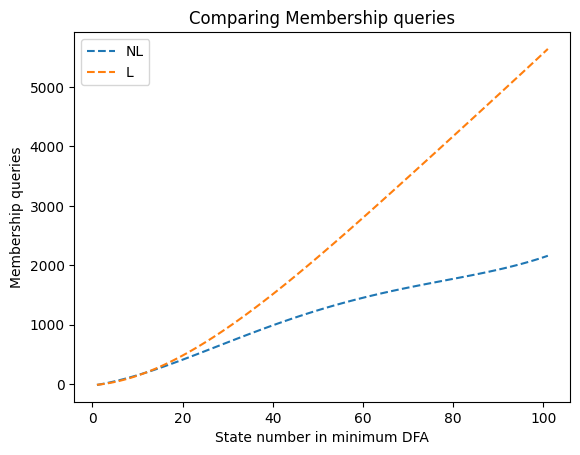
\includegraphics[width=\textwidth]{../statistics/plots/BenchMark/Membership queries.png}
    \caption{Membership queries Number}
    \label{fig:MemberBenchMarkCompare}
  \end{subfigure}
  \begin{subfigure}[b]{0.3\textwidth}
    \includegraphics[width=\textwidth]{../statistics/plots/BenchMark/Equivalence queries.png}
    \caption{Equivalence queries Number}
    \label{fig:EquivBenchMarkCompare}
  \end{subfigure}
  \begin{subfigure}[b]{0.3\textwidth}
    \includegraphics[width=\textwidth]{../statistics/plots/BenchMark/Transition nb in A.png}
    \caption{Transition Number}
    \label{fig:TransitionBenchMarkCompare}
  \end{subfigure}
  \begin{subfigure}[b]{0.3\textwidth}
    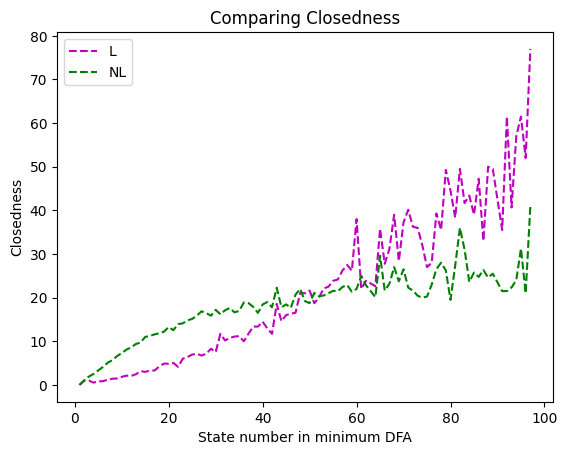
\includegraphics[width=\textwidth]{../statistics/plots/BenchMark/Closedness.png}
    \caption{Closedness Problem Number}
    \label{fig:ClosednessBenchMarkCompare}
  \end{subfigure}
  \begin{subfigure}[b]{0.3\textwidth}
    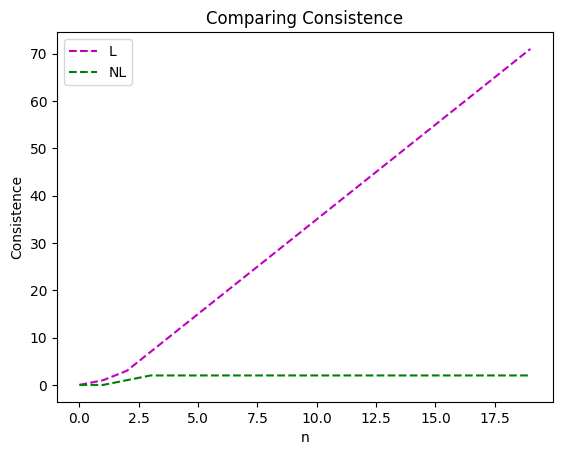
\includegraphics[width=\textwidth]{../statistics/plots/BenchMark/Consistence.png}
    \caption{Consistence Problem Number}
    \label{fig:ConsistenceBenchMarkCompare}
  \end{subfigure}
  \caption{mDFA vs cRFSA on random Teachers}
  \label{fig:benchmark}
\end{figure}

We see in \cref{fig:benchmark} that the number of states of \textit{cRFSA} is in general exponentially smaller than the \textit{mDFA} and that, concerning the number of equivalence and membership queries, the \textit{NL*} algorithm outperforms \textit{L*}. As expected the number of Consistence problems is won by the \textit{NL*} but curiously the Closedness comparison is taken by the \textit{NL*} only after about $50$ states.

Looking \cref{fig:MemberBenchMarkCompare} and \cref{fig:EquivBenchMarkCompare}, I can see that the gap between the \textit{NL*} and the \textit{L*} curves is not really big. Again, as for the previous section, when dealing with Teacher which demands a similar number of Membership and Equivalence problem for both \textit{NL*} and \textit{L*}, then it is the \textit{NL*} algorithm which will have more Closedness problems since to find all state of the \textit{Prime} residuals of the automaton it will have to promote more rows, thing that is more efficiently done by \textit{L*} which adds the counter-example in $S$.

In \cref{fig:TransitionBenchMarkCompare} we see that the number of transitions of the \textit{mDFA} is linear to the number of its states\footnote{Number of transitions $= |Sigma| \times$ number of states of the Automaton}, but the number of transitions in the \textit{cRFSA} is very often bigger. This is due to the fact that the \textit{cRFSA} tends to create a lot of transitions, sometimes redundant, from a state $q_i$ to every state $q_i'$ where $L(q_i') \subseteq L(q_i)$.

\section{Some curiosity about the two algorithms}

While discussing with my supervisors or coding the algorithms we have seen that the \textit{L*} or the \textit{NL*} algorithms can have some curious properties.

\subsection{Minimize an automaton}

If in a certain way, we merge the notion of Teacher and Learner L* together we can create an algorithm \textit{Minimizer} to calculate \textit{mDFA} of a general \textit{DFA}. The \textit{Minimizer} will be composed by the L* implementation and a second part able to compare two automata and provide as the Teacher a counter-example.

We have seen that if we create a \textit{Minimizer} the algorithm will be something like this:

\begin{algorithm}[h]
  \caption{Minimizer}
  \KwIn{An automaton $\A$}
  \KwOut{$\A$ minimized}

  \While{True}{
    Run L*\;
    \uIf{Membership Query}{
      Check if $\omega$ is accepted by L*;
    }
    \Else{
      Check the equivalence between the conjecture $\A'$ and the $\A$\;
      \uIf{Equivalence}{
        \Return $\A'$
      } \Else {
        Find a counter-example
      }
    }
  }
\end{algorithm}

% This algorithm is correct since \textit{L*} always return a \textit{mDFA} that recognizes a language $\U$ and the automaton passed in parameter can be see as the representation of a regular language $\U$, by \cref{th:kleene}.

% The algorithm terminates: \textit{L*} and verifying the equivalence of two automata terminate.

The time complexity is a bit more complicated to calculate. Let $N$ the size of the automaton passed in parameter and $n$ the size of its \textit{mDFA}. Then at most \textit{L*} will create $n$ conjectures, one per state of the \textit{mDFA}. So we will pass through the loop $n$ times. The complexity of the equivalence test between automata is at most:
\begin{itemize}
  \item $O(n)$ to make to complementation of an automaton of size $n$;
  \item $O(n \times m)$ to calculate the intersection of two automata of size $n$ and $m$;
  \item $O(n)$ to test if the automaton is empty or find a counter-example.
\end{itemize}
The equivalence ask for:$(\LA \cap \overline{\mathcal{L}(\A')}) \cup (\overline{\LA} \cap \mathcal{L}(\A'))$ and applying the previous complexity asks $O(2 \times (N + n + N \times n)) = O(n \times N)$.

The Learner complexity is $O(n^3)$ because the size of the longest counter-example will be at most $n$\footnote{The counter-example will always be of least length}.

The overall complexity inside the loop is $O(n)*(O(n^3) + O(n \times N)) = O(n^4 + n \times N)$.

A good algorithm that we know to minimize an automaton takes $O(N \log(N))$ which is clearly better than the \textit{Minimizer} complexity, however the \textit{Minimizer} can be better if the automaton to minimize has a very huge number of states and its minimized version is very small.

We can also create an \textit{NL-Minimizer} but in this case we will work with \underline{non} deterministic automata and the operation of complementation on that kind of automata is an hard problem.

\subsection{Can we remove the Consistence check?}

While testing the performances of the Learners algorithms, I have tried to modified some of their properties to see their behavior. For example I have seen that \textit{Consistence} if we remove the consistence check on the \textit{NL*} algorithm the algorithm seems to terminates on every expression of the benchmark sample, even if I do not have a concrete proof. I think that adding the counter-example into $E$ will autonomously allow to add the necessary columns to find the \textit{Prime} residuals.

In fact the consistence check allows to add new columns, but if we do not add this constraints, we will send conjectures when the table is only closed and the next counter-example will allow to spot new residuals.

The main drawback of this approach is that the Learner will have to make more Equivalence queries which, as said in \cref{sec:worstRFSA}.
